\section{輕重鍊剖分}
    \subsection{概念}
    輕重鍊剖分是樹上的特殊方法,他可以藉由預處理的方式,將查詢
    區間最大最小值與區段總和的時間複雜度降到$O(\log^{2}{(n)})$以下,
    相較於原來的$O(n)$而言會快上許多。

    首先同樣要先定根,接著我們透過一次DFS確定每個節點的子樹大小。

    在輕重鍊剖分中,我們會優先從子樹最大的節點往下連接,又稱為重邊
    ,而其他的邊則稱為輕邊。這樣可以保證我們的鍊的數量不會超過$O(\log{(n)})$條。

    \begin{figure}[h]
        \centering
        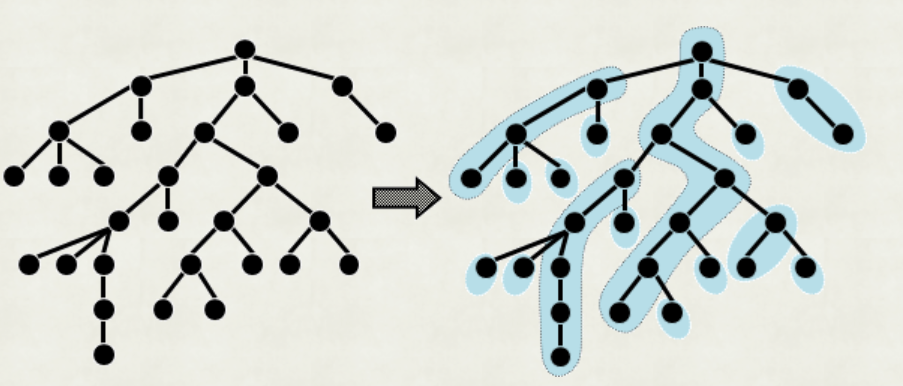
\includegraphics[width=\textwidth]{../Images/HLD.png}
        \caption{輕重鍊剖分示意圖}
    \end{figure}

    \subsection{實作}
    實作上我們會需要很多個陣列。

\begin{lstlisting}[caption=輕重鍊剖分與線段樹]
using ll=long long;
const int N=100010;
const ll INF=0x3f3f3f3f3f3f3f3f;
using pii=pair<int,int>;

int sz[N],fa[N],to[N],fr[N],dep[N],dfn[N];
// sz[x]  = x 的子樹大小
// fa[x]  = x 的 parent node
// to[x]  = x 所有子節點中,子樹最大的
// dep[x] = x 到根的距離
// dfn[x] = dfs(x)時的標記
// fr[x]  = x 所在的鍊的頭

int n;
vector<int> g[N];

void dfs(int x,int p){
    sz[x]=1, fa[x]=p, to[x]=-1;
    dep[x]=(p!=-1) ? dep[p]+1 : 0;

    for(auto u:g[x]) if(u!=p){
        dfs(u,x);
        sz[x]+=sz[u];
        if(to[x]==-1 || sz[u]>sz[to[x]])
            to[x]=u;
    }
}

void link(int x,int f){
    // time stamp
    static int tk=1;
    fr[x]=f;
    dfn[x]=tk++;// dfn[x]=tk, tk++;
    // extend the chain
    if(to[x]!=-1) link(to[x],f);

    for(auto u:g[x]){
        if(u==fa[x] || u==to[x]) continue;
        link(u,u);
    }
}

vector<pii> QueryPath(int u,int v){
    // return the intervals on the path from u to v
    int fu=fr[u],fv=fr[v];
    vector<pii> ret;
    while(fu!=fv){
        if(dep[fu]<dep[fv])
            swap(fu,fv), swap(u,v);
        ret.emplace_back(dfn[fu],dfn[u]);
        u=fa[fu];
        fu=fr[u];
    }
    if(dep[u]>dep[v]) swap(u,v);
    // now u is LCA
    ret.emplace_back(dfn[u],dfn[v]);
    return ret;
}

struct Seg{
    struct node{
        ll val,tag;

        node *rch,*lch;
        
        node(){
            val=tag=0;
            rch=lch=nullptr;
        }

        node(ll v){
            val=v, tag=0;
            rch=lch=nullptr;
        }

        void push(int l,int r){
            int len=r-l+1>>1;
            if(lch){
                lch->val+=tag*len;
                lch->tag+=tag;
            }
            
            if(rch){
                rch->val+=tag*len;
                rch->tag+=tag;
            }
            tag=0;
        }
        
        void pull(){
            val=0;
            if(lch) val+=lch->val;
            if(rch) val+=rch->val;
        }

        void modify(int p,ll v,int lb=1,int rb=n){
            if(lb==rb){
                val=v;
                return;
            }

            if(!lch) lch=new node();
            if(!rch) rch=new node();

            push(lb,rb);
            
            int mid=lb+rb>>1;

            if(p<=mid) lch->modify(p,v, lb ,mid);
            if(mid<p)  rch->modify(p,v,mid+1,rb);

            pull();
        }

        ll query(int l,int r,int lb=1,int rb=n){
            if(l<=lb && rb<=r){
                return val;
            }

            push(lb,rb);
            
            int mid=lb+rb>>1;

            ll ret=0;
            if(lch && l<=mid) ret+=lch->query(l,r, lb ,mid);
            if(rch && mid<r)  ret+=rch->query(l,r,mid+1,rb);

            pull();

            return ret;
        }
        
        void add(int l,int r,ll v,int lb=1,int rb=n){
            if(l<=lb && rb<=r){
                val+=v*(rb-lb+1);
                tag+=v;
                return;
            }

            push(lb,rb);
            
            int mid=lb+rb>>1;

            int ret=0;
            if(lch && l<=mid) lch->add(l,r,v, lb ,mid);
            if(rch && mid<r)  rch->add(l,r,v,mid+1,rb);

            pull();
        }
    };

    node *rt=new node();//root

    void modify(int p,int v){
        rt->modify(p,v);
    }

    ll query(int l,int r){
        return rt->query(l,r);
    }

    void add(int l,int r,ll v){
        rt->add(l,r,v);
    }
};

Seg seg;

void modify(int v,int p){
    p=dfn[p];
    seg.modify(v,p);
}

ll query(int u,int v){
    vector<pii> pt=QueryPath(u,v);
    ll ret=0;
    for(auto p:pt){
        ret+=seg.query(p.first,p.second);
    }
    return ret;
}

ll add(int u,int v,ll k){
    vector<pii> pt=QueryPath(u,v);
    for(auto p:pt){
        seg.add(p.first,p.second,k);
    }
}
\end{lstlisting}

    \subsection{範例與練習}
    \problem 第一屆卓越盃 G. Safe Tariff(Hard)

    \textbf{題目敘述}

    太平洋上有 $n$ 個島嶼國家,為了方便起見將其命名為 $1$ ~ $n$ 。
    這些島嶼國家皆使用一個共同貨幣,他們稱其為國際銀幣。
    各個國家之間有許多貿易往來,其中一種便是金磚航運。
    並且在這些國家之間有一些固定的航線往來,這些航線也是交流與物產貿易的主要手段。
    每一條航線都是往返固定兩個國家。若一航線是往返國家 $u$ ,
    則以 $(u,v)$ 或 $(v,u)$ 表示該航線,兩種表示方法相同,
    代表聚客 $u$ 與國家 $v$ 可以直航交易兩地。
    如果國家 $u$ 與國家 $v$之間沒有航線直接往返也可能透過複數航線進行貿易。
    若存在一系列的航線 $(u,p_1),(p_1,p_2) . . . (p_r,v)$ 則國家 $u$ 與國家 $v$ 之間便可以進行貿易,
    反之則不行。

    為了保護太平洋的生態,所有國家的共識是在任兩個島嶼國家之間都能夠進行貿易往來的前提下維持
    盡可能少的航線。顯而易見的,在 $n$ 個國家的情況下僅需要 $n-1$ 條航線就足夠了。

    每個國家為了保護自己內部的產業不受到外部的低價商品傾銷、惡性競爭。
    因此對各項商品都設定有關稅。而在太平洋上關稅課徵的方式是針對貨物數量,
    在每一航線上船上所装載的商品都要被抽一次税金。依據商品的種類不同有不同的抽税方式;
    而針對金磚,則是每一個保險箱要課徵 $c$ 個國際銀幣。
    然而因為金磚航運生意普普,因此\textbf{所有}國家起初並不是非常重視,
    也就沒有對其課徵關稅。

    黃瓜學長是一個專做金磚航運的 \textbf{``為何年輕人都不愛讀近體詩"} 企業的老闆,
    客戶所在的國家與當下金磚能出貨的國家不同,可能會被課徵關稅也不同。
    他希望可以收取合理的價格以避免無法獲利,或是被投訴價格過高不符合公平貿易。
    因此他需要計算航線上會被課徵多少關稅。

    並且,由於最近發生金融危機,加上疫情高漲,許多原來不課徵關稅的國家也嗅到了這股商機,
    選擇開始課徵關稅。所以黃瓜學長必須隨時調整售價來因應關稅的變動。
    以免傷害到 \textbf{``為何年輕人都不愛讀近體詩"} 的競爭力。

    \textbf{輸入說明}

    第一行輸入 $2$ 個數字 $n$ $q$ ,代表有 $n$ 個國家, $q$ 次操作
    
    接下來有 $n-1$ 行,每行有 $2$ 個數字 $u$ $v$ ,代表國家 $(u,v)$ 之間有直接的航道。
    
    接下來有 $q$ 行,每行有 $3$ 個數字 $op$ $a$ $b$
    
    若 $op=1$ ,代表黃瓜學長收到訂單(從國家 $a$ 輸送到國家 $b$ )
    
    否則 $op=2$ ,代表國家 $a$ ,將關稅改為 $b$ 國際銀幣/保險箱
    
    $op \in \text{{1,2}}$,$n,q$ $\leq 10^5$,$a,b \le n$

    \textbf{輸出說明}

    對於 $op==1$ 輸出所需關稅(輸出國 $(a)$ 不會課關稅,但輸入國 $(b)$ 會)。

    \textbf{範例測試}

    \begin{tabular}{|m{7cm}|m{7cm}|}
        \hline
        範例輸入 1 & 範例輸出 1 \\
        \hline
        \verb|7 10|  & \verb|0| \\
        \verb|6 5|   & \verb|0| \\
        \verb|7 5|   & \verb|0| \\
        \verb|4 3|   & \verb|0| \\
        \verb|4 5|   & \verb|207| \\
        \verb|4 2| & \\
        \verb|6 1| & \\
        \verb|1 3 7| & \\
        \verb|1 3 1| & \\
        \verb|2 6 207| & \\
        \verb|1 7 4| & \\
        \verb|1 6 4| & \\
        \verb|2 2 683| & \\
        \verb|2 3 119| &  \\
        \verb|1 5 6| &  \\
        \verb|2 1 579| &  \\
        \verb|2 1 947| & \\
        \hline
    \end{tabular}

    \problem 洛谷P2680 運輸計畫

    \textbf{題目敘述}

    公元 2044 年,人類進入了宇宙紀元。

    L 國有 $n$ 個星球,還有 $n-1$ 條雙向航道,每條航道建立在兩個星球之間,這 $n-1$ 條航道連通了 L 國的所有星球。

    小 P 掌管一家物流公司,該公司有很多個運輸計劃,每個運輸計劃形如:有一艘物流飛船需要從 $u_i$ 號星球沿最快的宇航路徑飛行到 $v_i$ 號星球去。顯然,飛船駛過一條航道是需要時間的,對於航道 $j$,任意飛船駛過它所花費的時間為 $t_j$,並且任意兩艘飛船之間不會產生任何干擾。

    為了鼓勵科技創新,L 國國王同意小 P 的物流公司參與 L 國的航道建設,即允許小 P 把某一條航道改造成蟲洞,飛船駛過蟲洞不消耗時間。

    在蟲洞的建設完成前,小 P 的物流公司就預接了 $m$ 個運輸計劃。在蟲洞建設完成後,這 $m$ 個運輸計劃會同時開始,所有飛船一起出發。當這 $m$ 個運輸計劃都完成時,小 P 的物流公司的階段性工作就完成了。

    如果小 P 可以自由選擇將哪一條航道改造成蟲洞,試求出小 P 的物流公司完成階段性工作所需要的最短時間是多少?

    \textbf{輸入說明}

    第一行包括兩個正整數 $n, m$,表示 L 國中星球的數量及小 P 公司預接的運輸計劃的數量,星球從 $1$ 到 $n$ 編號。

    接下來 $n-1$ 行描述航道的建設情況,其中第 $i$ 行包含三個整數 $a_i, b_i$ 和 $t_i$,表示第 $i$ 條雙向航道修建在 $a_i$ 與 $b_i$ 兩個星球之間,任意飛船駛過它所花費的時間為 $t_i$。

    接下來 $m$ 行描述運輸計劃的情況,其中第 $j$ 行包含兩個正整數 $u_j$ 和 $v_j$,表示第 $j$ 個運輸計劃是從 $u_j$ 號星球飛往 $v_j$號星球。

    數據保證 $1 \leq a_i,b_i \leq n$,$0 \leq t_i \leq 1000$,$1 \leq u_i,v_i \leq n$
    
    \textbf{輸出說明}

    一個整數,表示小 P 的物流公司完成階段性工作所需要的最短時間。

    \textbf{範例測試}

    \begin{tabular}{|m{7cm}|m{7cm}|}
        \hline
        範例輸入 1 & 範例輸出 1 \\
        \hline
        \verb|6 3|   & \verb|11| \\
        \verb|1 2 3| & \\
        \verb|1 6 4| & \\
        \verb|3 1 7| & \\
        \verb|4 3 6| & \\
        \verb|3 5 5| & \\
        \verb|3 6| & \\
        \verb|2 5| & \\
        \verb|4 5| & \\
        \hline
    \end{tabular}

    \begin{tip}
        需要快讀快寫,記得往前翻。
    \end{tip}